\documentclass[12pt]{article}
\usepackage[utf8]{inputenc}
\usepackage[T2A]{fontenc}
\usepackage[mongolian]{babel}
\usepackage{graphicx}
\graphicspath{{image/}}
\begin{document}
	\section{Функциональ шаардлага:}
	\begin{enumerate}
		\item Оюутан бүртгэх
		\item Зар бүртгэх
		\item Төлөвлөгөө бүртгэх
		\item Дүнгийн мэдээлэл
		\item Зарын мэдээлэл
		\item Оюутанын мэдээлэл
		\item Хайлт хийх
		\item Зарын дагуу оюутан бүртгэнэ
		\item Оюутан хайна
		\item Багшийн мэдээлэл
		\item Оюутаны мэдээлэл хардаг байх
		\item Оюутаны хичээлийн хуваарь хардаг байх
		\item Эцэг эхийн мэдээлэл хардаг байх
		
	\end{enumerate}
	
	\section{Функционал бус шаардлага}
	\begin{enumerate}
		\item Дүнгийн мэдээлэл хараад лимит тогтооно
		\item Мэдээлэл хайхад хурдацтай байх
		\item Кодчилолын хувьд CodeIgniter framework –ийн стандартын дагуу хийгдэнэ.
		\section{Юзкэйс диаграм}
		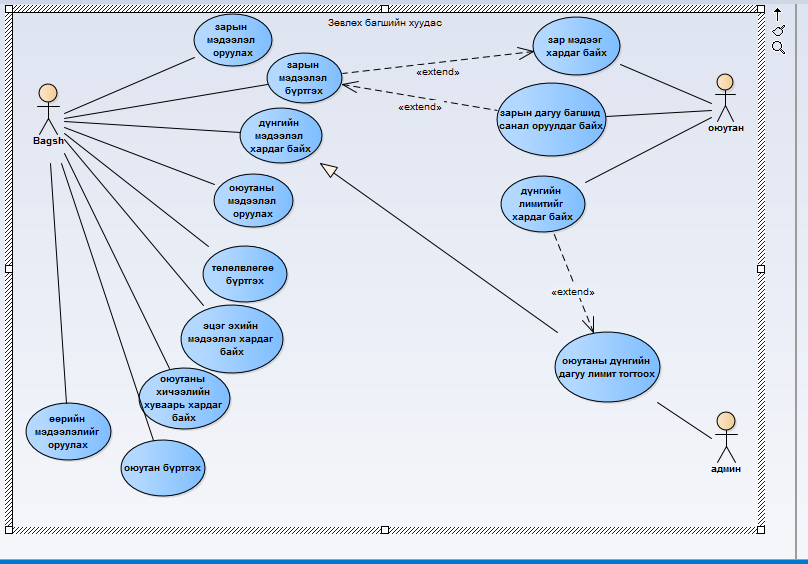
\includegraphics[scale=0.6]{usecase5}
		\section{Sequence диаграм}
		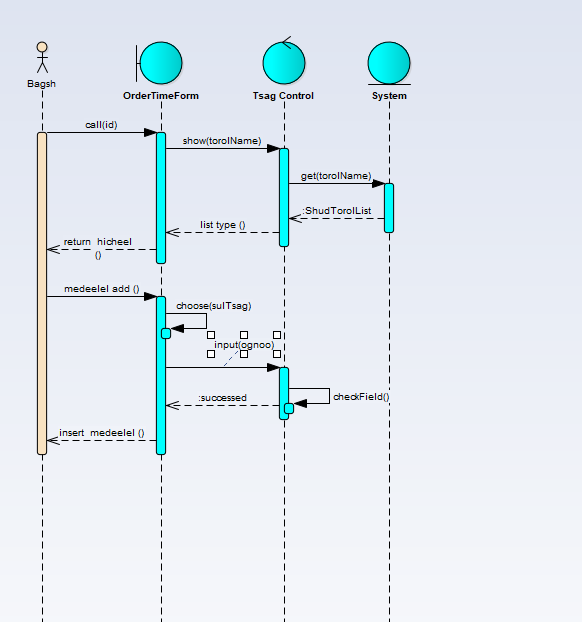
\includegraphics[scale=0.6]{sequence.png}
		\section{Класс диаграм}
		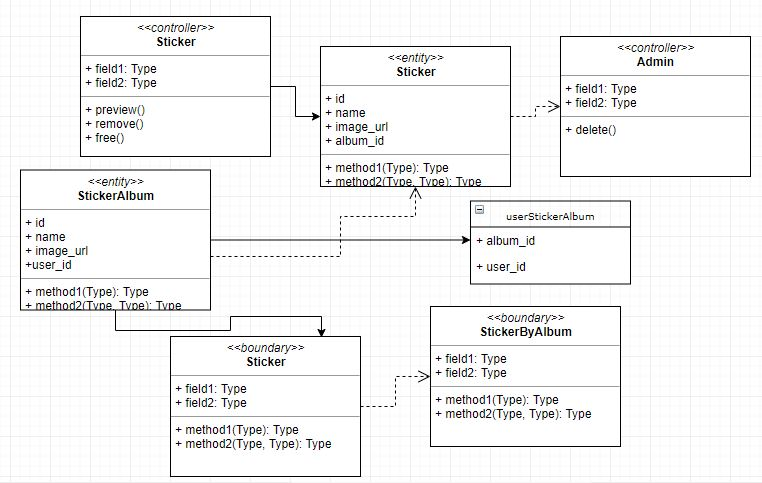
\includegraphics[scale=0.6]{class.png}
		\section{activity диаграм}
		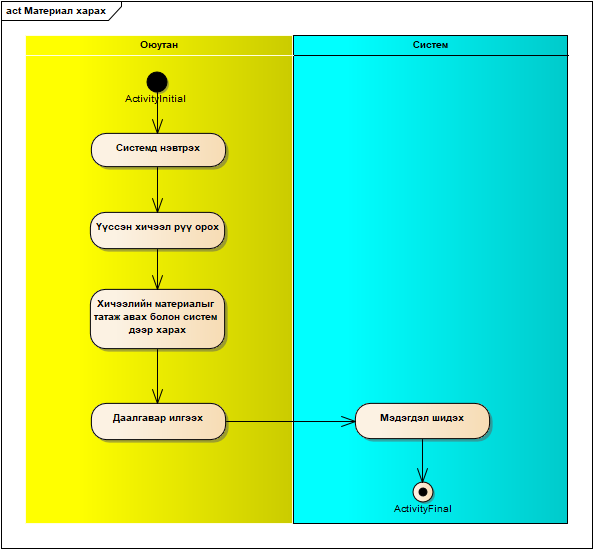
\includegraphics[scale=0.6]{activity.png}
	\end{enumerate}
\end{document}


